\subsection{QuizziPedia::Back-End::App::Controllers}
\label{QuizziPedia::Back-End::App::Controllers}
\begin{figure}
	\centering
	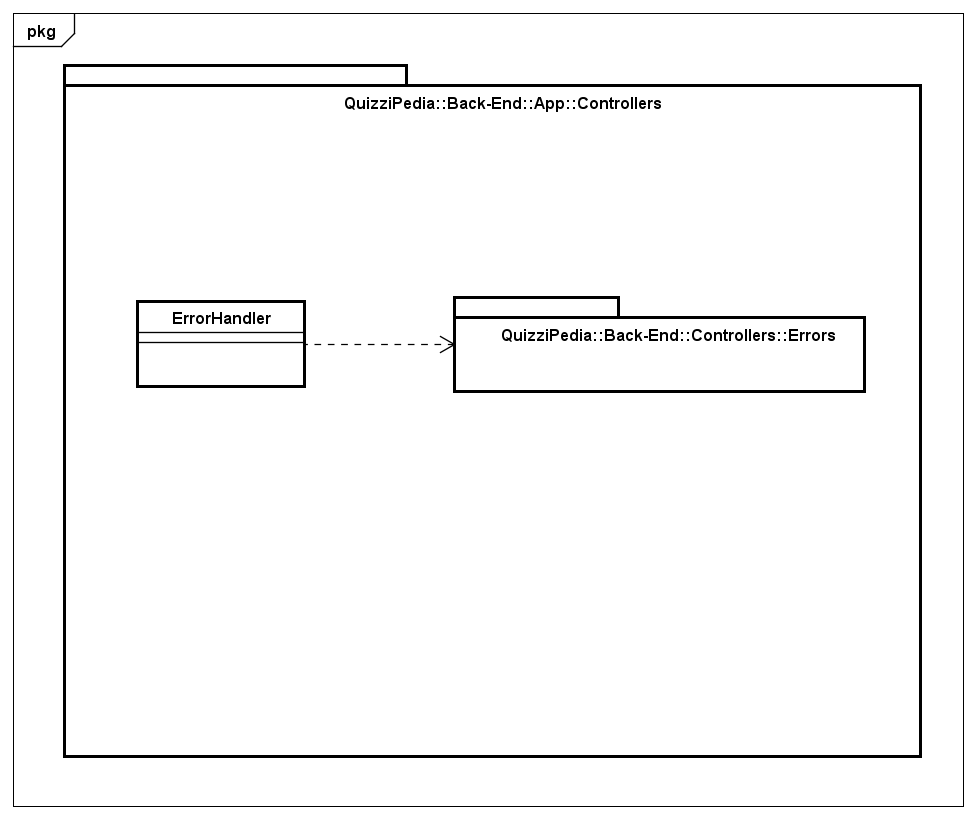
\includegraphics[scale=0.45]{UML/Package/QuizziPedia_Back-End_App_Controllers.png}
	\caption{QuizziPedia::Back-End::App::Controllers}
\end{figure}
\subsubsection{Informazioni generali}
	\begin{itemize}
		\item \textbf{Descrizione} \\
		Package contenente i controllers di Express, definisce la logica dell'applicazione.
		\item \textbf{Padre}: \texttt{App}
		\item \textbf{Interazioni con altri componenti}
			\begin{itemize}
				\item \texttt{Routers} \\
				Package contenente i router della componente back-end dell'applicazione. Contiene i file di configurazione relativi al routing delle richieste del client, ossia i routers di Express.
				\item \texttt{Views} \\
				Package contenente le views della copmonente back-end dell'applicazione.
			\end{itemize}
		\item \textbf{Package contenuti}:
			\begin{itemize}
				\item \texttt{Errors} \\
				Package contenente i controllers per la gestione degli errori specifici.
			\end{itemize}
	\end{itemize}
\subsubsection{Classi}
\paragraph{QuizziPedia::Back-End::App::Controllers::ErrorsHandler}
\begin{itemize}
	\item \textbf{Descrizione}:\\
	Classe middleware per la gestione degli errori. Ritorna al client un oggetto di tipo Response con stato HTTP 500 e descrizione dell’errore in formato JSON. È un componente ConcreteHandler del design pattern Chain of responsibility.
	\item \textbf{Utilizzo}:\\
	Viene utilizzata quando si verifica un errore. Si preoccupa di delegare la costruzione del messaggio d’errore al modulo specifico qualora questo esista, altrimenti costruisce un messaggio d’errore generico. In questo modo i messaggi d’errore specifici vengono delegati ad un altro modulo, rendendo così possibile aggiungere in futuro altri moduli per gestire più flessibilmente nuove tipologie di errori.
	\item \textbf{Relazioni con altre classi}:\\
	\begin{itemize}
		\item ................
		\item OUT \texttt{QuizziPediaError}\\
		Classe di gestione degli errori. Esegue la costruzione del messaggio d’errore specifico per i moduli di Premi::Back-End::App.
	\end{itemize}
	\item \textbf{Metodi}:\\
	\begin{itemize}
		\item \texttt{+ handleError(err: QuizziPediaError, req: Request, res: Response, next: function(QuizziPediaError))}\\
		Metodo che gestisce la costruzione dei messaggi d’errore ritornando un JSON contenente il messaggio d’errore.\\
		\textbf{Parametri}:
		\begin{itemize}
			\item \texttt{err: QuizziPediaError}\\
			Rappresenta l'errore di tipo \texttt{QuizziPediaError}.
			\item \texttt{req: Request}\\
			Rappresenta la richiesta inviata al server.
			\item \texttt{res: Response}\\
			Rappresenta la risposta che il server fornirà al termine dell'esecuzione del metodo.
			\item \texttt{next: function(QuizziPediaError)}\\
			Rappresenta la \textit{callback\ped{G}} che il metodo deve chiamare al termine dell’elaborazione per passare il controllo ai successivi middleware. La presenza del parametro facoltativo QuizziPediaError attiva la catena di gestione dell’errore in sostituzione della normale catena di gestione delle richieste.
		\end{itemize}
	\end{itemize}
\end{itemize}
\paragraph{QuizziPedia::Back-End::App::Controllers::NOMECLASSE}
\begin{itemize}
	\item \textbf{Descrizione} \\
	\item \textbf{Utilizzo} \\
	\item \textbf{Relazioni con altre classi} \\
	\item \textbf{Metodi} \\
\end{itemize}